\documentclass[tikz,border=10pt]{standalone}
\usepackage{pgfplots}
\pgfplotsset{}
\usepackage{booktabs}

\begin{document}

% Begin the figure environment
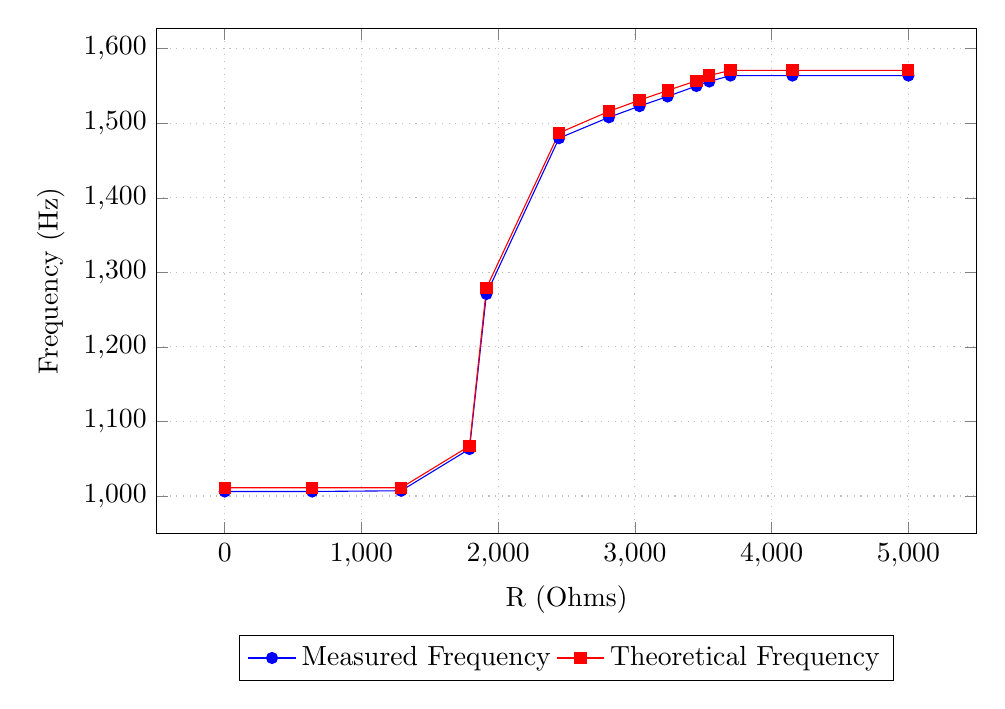
\begin{tikzpicture}

% Define the table and plot layout
\begin{axis}[
    width=12cm,
    height=8cm,
    grid=both,
    grid style={dotted},
    xlabel={R (Ohms)},
    ylabel={Frequency (Hz)},
    legend style={at={(0.5,-0.2)}, anchor=north, legend columns=-1},
    legend entries={Measured Frequency, Theoretical Frequency},
    legend cell align={left}
]

% Measured Frequency Plot
\addplot[color=blue, mark=*] table {
0    1006
640  1006
1290 1007
1790 1063
1914 1271
2445 1480
2810 1508
3034 1523
3239 1536
3450 1550
3544 1556
3699 1564
4152 1564
5000 1564
};

% Theoretical Frequency Plot
\addplot[color=red, mark=square*] table {
0    1011
640  1011
1290 1011
1790 1067
1914 1279
2445 1487
2810 1516
3034 1531
3239 1544
3450 1557
3544 1564
3699 1571
4152 1571
5000 1571
};

\end{axis}
\end{tikzpicture}

% Create the table below the plot
\[
\begin{array}{ccc}
\toprule
\textbf{R (Ohms)} & \textbf{Theoretical Frequency (Hz)} & \textbf{Measured Frequency (Hz)} \\
\midrule
0    & 1011 & 1007 \\
640  & 1011 & 1007 \\
1290 & 1011 & 1007 \\
1790 & 1067 & 1064 \\
1914 & 1279 & 1272 \\
2445 & 1487 & 1481 \\
2810 & 1516 & 1509 \\
3034 & 1531 & 1524 \\
3239 & 1544 & 1537 \\
3450 & 1557 & 1551 \\
3544 & 1564 & 1557 \\
3699 & 1571 & 1565 \\
4152 & 1571 & 1565 \\
5000 & 1571 & 1565 \\
\bottomrule
\end{array}
\]

\end{document}
